\chapter{Orientation} \label{cha:orientation}
\pagenumbering{arabic}
	This chapter provides an overview of the orientation phase of the project,
	as well as giving an overview of the entire process of the project from start to finish.
	It shows an analysis of the project requirements, and the decisions that
	have been made during the project regarding choices of frameworks and
	libraries as well as game play elements. It also functions as a thorough
	introduction to this report.

	For a more in-depth view on the research that has been done leading to
	these decisions, please refer to the Research Report in appendix
	\ref{app:researchreport}.

	\section{Project Description} \label{sec:projectdescription}
		While augmented reality research has grown into a mature field over the
		last years, the aspects of situational awareness and presence of
		augmented reality (AR) are still quite open research topics. This
		project is about designing and implementing a collaborative game to
		explore the different perception of situational awareness, presence and
		workload in a physical and an AR environment. The game is to be employed
		as an approximation of collaboratively solving complex problems, as they
		occur in crime scene investigation when using virtual co-location, i.e.
		remote crime scene experts to guide local investigators in
		AR to collaboratively analyze the crime scene.

	\section{Final Product} \label{sec:finalproduct}
		The goal of the game is to solve a puzzle by controlling laser beams
		using mirrors in such a way that a predefined target is hit. The game
		can be played by one or more local players and one or more remote players.
		
		There are cards present for the local players that represent mirror
		bases. These must be placed on the table, which will be the locations
		for the mirrors. The local players will be able to see the mirrors they
		place through the use of AR technology. Each of the local players will
		only be given a few of the mirror bases needed to solve the puzzle, and
		as such solving it requires cooperation from all local players.
		
		The remote players can also see the placed mirrors, and can rotate them
		to influence the path of the laser beam(s). Only by cooperation between
		local players (who can only move the mirror bases) and remote players
		(who can only rotate them) it becomes possible to hit the target and as
		such solve the puzzle.
		
		The game provides various types of objects with different capabilities, 
		allowing for more complex puzzles. Examples of such objects include,
		but are not limited to walls, laser beam splitters and checkpoints.
		For a complete overview of the game objects provided by the game, see
		section \ref{sec:graphicaldesign}.
		
		The game is designed to stimulate cooperation between physically
		co-located players and the remote player(s). It does so by
		dividing abilities required for solving the puzzles amongst all players
		as follows:
		
		\begin{itemize}
			\item Physically co-located players each get only a part of the
			mirror bases required to solve the puzzle, requiring input
			from all of these players.
			\item Physically remote players have the ability to rotate
			mirrors while the physically co-located players do not have
			this ability, requiring input from both physically co-located
			as well as remote players.
		\end{itemize}
	
	\section{Software Design Methods} \label{sec:designmethods}
		This section describes the design methods that were used during the
		project. It illustrates the methodology that was used to develop and
		coordinate the project during the development phase.
	
		\subsection{Design Process} \label{ssec:designprocess}
			In designing and implementing the product, it is important that
			requirements can be changed quickly and without much problems. This is
			not because the requirements are likely to change from the client
			side, but because the choice of AR technology may change over the
			course of the project because of technical issues. The available Virtual
			and Augmented Reality glasses are mostly still in development, and as
			such this may affect the technical viability of each device.
			
			To deal with such changes, we use the Scrum methodology \cite{scrum}. This
			methodology describes a set of rules that, amongst others, makes it
			easier to deal with various changes during the development process.
			The methodology
			in graph form can be seen in \ref{fig:scrum}. The methodology
			shown is nearly identical to what we use, the only 
			exception being that our sprints only last one week instead of two.
			
			\begin{figure}
			\centering
			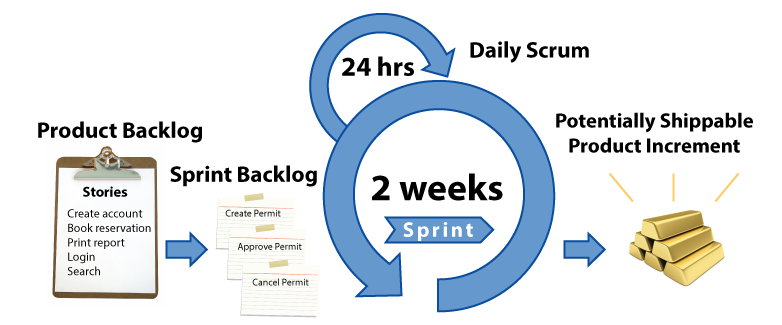
\includegraphics[width=\textwidth]{Scrum}
			\caption{Scrum methodology overview}
			\label{fig:scrum}
			\end{figure}
		
		\subsection{Organization} \label{ssec:organization}
			To be able to simultaneously work on the project without conflicts, we
			use Git as a version control system. The project is stored remotely on
			GitHub, ensuring the work is efficiently shared between all team members.
			Also, Git stores all commits that have been done. These can be reviewed
			on GitHub, and it is possible to go back to a commit stage if we
			absolutely need to, in case of something horribly wrong happening to
			the project.
			
			To coordinate and divide the tasks, as well as to maintain the items in
			the Scrum backlog, we use Trello. Trello is an on-line service that
			provides a dynamic way to organize items in various lists. It does
			so by using cards as bullet points in a list. It is also possible to
			assign certain people to those cards, which can be used to visibly
			divide tasks among the group members. Using labels, each card can also
			be categorized as a task relating to a certain part or parts of the
			project, such as software engineering, graphics design, networking,
			etc. We created lists to keep track of which items were in the backlog, 
			which items were being worked on and which items were already done.
			This allowed us to easily see what was being done and what was done.
			
			The project is licensed under the terms of the MIT license. We chose
			this license because it allows other developers to learn from this
			project. Additionally, since this project is done as a part of a
			research project, we believe making it open source may
			help future researchers in the same field. The full terms of the MIT
			license can be found at \url{http://opensource.org/licenses/mit-license.html}
			
			%TODO Move this paragraph to correct sections in the Quality Assurance chapter.
			To ensure the C\# source code in the project meets common coding standards
			(as set by Microsoft), we use the code analysis tools FxCop and StyleCop
			in combination with SonarQube. FxCop performs static code analysis, like
			code complexity and some naming conventions. StyleCop, on the other hand,
			focuses more on code style which includes use of spacing and
			documentation as well as other factors. SonarQube is a platform that
			unifies the reports from these tools and provides a clean overview of the
			combined issues found by FxCop and StyleCop, as well as some simple metrics
			SonarQube has built-in. Further detail about maintaining code quality
			is described in the QA section of the report, chapter 4.
			
		\subsection{Design Architecture} \label{ssec:designarchitecture}
			Because the product is a game and the goal of the project is more
			focused on the game mechanics rather than the underlying engine, we chose
			to use Unity as a starting point. Unity provides a platform independent
			development environment for creating games, and offers many features 
			commonly used in games.
			
			Using Unity means that the project architecture is bound to the
			loosely coupled component-based architecture that Unity provides,
			although it is possible to include principles from object-oriented
			programming to some extent.
			
		\section{Process}\label{sec:process}
			This section describes the process of the project. The different phases
			during the project are highlighted in this section.
		
		\subsection{Early Preparations} \label{ssec:preparations}
			Before the project started, we had a meeting halfway through March
			with our coach about what the project entails and what is currently
			possible, given the hardware that we have today. After a brainstorm
			session and a pitch session with our coach and client, we were shown 
			what kind of hardware the TU Delft has available, and also what the 
			limitations of this hardware are. In this phase, a product plan was
			also created. This document describes the planning for the duration
			of the project, and can be found in appendix \ref{app:productplan}.
		
		\subsection{Research} \label{ssec:research}
			The first two weeks were the main research phase. This entailed that the
			research report had to be written. The second week was partly devoted
			to writing the report, and also to testing out more functionality of
			the software and hardware. The first game object models were also
			developed during this time, and there were plans for a first demo at the end
			of week 3 or at the beginning of week 4. The research report, which was the 
			result of these two weeks, can be found in appendix \ref{app:researchreport}
		
		\subsection{Programming the basic game} \label{ssec:basics}
			The next two weeks revolved around creating game objects and game play.
			After some testing with markers and AR glasses, as well game objects, a 
			first demo was also developed during this time. This phase also saw unit testing of game
			elements, as well as heavy usage of StyleCop and SonarQube to clean up
			respectively reorganize code in order to deliver clean code to SIG, for our first
			submission.  
		
		\subsection{The OpenCV server} \label{ssec:firstdemo}
			Week 5 finally saw the first demo being demonstrated to the coach. The
			coach was satisfied, but there was a lot to be done before the project
			could be considered finished. During this week, networking was revamped
			and development of a server that makes use of the computer vision library
			OpenCV started. This decision was based on various technical challenges we 
			came across during development. The reason for this decision can be found 
			in the Implementation chapter (chapter \ref{cha:implementation}).
		
		\subsection{Restructuring the entire project}
			Week 6 began with a massive restructuring of the project. Right before
			the code was to be handed in to SIG, Unity failed to build the project
			completely. There were no errors in the scripts, but the Unity compiler
			kept throwing unexplainable error messages. This caused us to move 
			everything that we wanted to move from the original project to a new
			Unity project.
			
			Even though this caused a setback in the project planning, this issue
			gave us an opportunity to take a critical look at our code base. After
			completing this task and handing in the package for SIG, development 
			could continue on the OpenCV server. The results for the SIG evaluation
			from this week can be found in appendix \ref{app:sig1}.
		
		\subsection{The new projection code}
			Week 7 began with further development on the OpenCV server and the code
			needed for correct projection of the META One. The projection code base
			was overhauled on Monday, mainly to allow for better unit testing. During
			this week, the midterm meeting also took place, and we could show off
			what we had up until that point. The coach and the customer(s) (Stephan
			could not be there, so he sent some of his colleagues to check in on
			how the project went) were impressed, but they also said that development
			had to continue for the time being. At the end of week 7, the server was
			completed, but now the true challenge began: integrating all the software
			into one single product.
			
			Week 8 started with the integration of all the parts of the software.
			From the start on, this proved quite challenging. Players could rotate
			mirrors by rotating the markers (which shouldn't happen, as this would
			kill off the co-operative element of the game), as well as other things.
			As such, development on projection code was once again necessary.
			Throughout this week, massive progress was made towards integration of 
			the various parts of the software, especially from early Wednesday on.
			Because of the progress considering integration of software, level design
			could finally start.
		 
		\subsection{Further integration}
			Week 9 was even further devoted to integration of all the various bits and
			pieces of the software. Once again, massive progress was made in
			integrating all software, and at the end of the week, the first fully
			working version was finally released. 
		 
		\subsection{Wrapping up}
			At the end of week 10, the final report had to be handed in. This meant
			that the project had to be wrapped up. The main activity in this week
			was testing with other users (the client and a few volunteers), as
			well as checking the final report before it had to be handed in.
			Also, the info sheet was written in this week, as it is required
			to have that checked before the final report can be handed in.
					 
		\subsection{The process table} \label{ssec:processtable}
			The following table gives a nice and short overview regarding what was done
			every week. An X in a particular subproject and week means that, during that
			week, that subproject was developed further.
			
			\begin{table}[!ht]                                                                                      
				\begin{tabular}{| c | c | c | c | c | c | c | c | c | c | c |}
				\hline
				Weeks             & 1      & 2      & 3      & 4      & 5      & 6      & 7      & 8      & 9      & 10     \\ \hline
				Research          & X      & X      & \space & \space & \space & \space & \space & \space & \space & \space \\ \hline
				Final report      & \space & \space & \space & X      & X      & X      & X      & X      & X      & X \\ \hline
				Networking        & X      & X      & \space & \space & X      & X      & X      & \space & X      & X \\ \hline
				Augmented reality & \space & \space & \space & X      & X      & X      & X      & X      & \space & \space \\ \hline
				Game elements     & X      & X      & X      & X      & \space & \space & \space & \space & \space & \space \\ \hline
				Testing           & \space & \space & X      & X      & X      & X      & X      & X      & \space & X \\ \hline
				Projection        & \space & \space & \space & X      & X      & X      & X      & X      & X      & \space \\ \hline
				Level design      & \space & \space & \space & \space & \space & \space & \space & X      & X      & X \\ \hline
				\end{tabular}
			\end{table}
